\documentclass[tikz,border=10pt]{standalone}
\usepackage{tikz}
\usepackage{amsmath,amssymb}
\usepackage{fontawesome5}
\usetikzlibrary{arrows.meta,positioning,fit,backgrounds,calc,shadows,shapes.geometric}

% Color definitions
\definecolor{lavenderDark}{RGB}{15, 44, 89}
\definecolor{lavenderDeep}{RGB}{10, 28, 58}
\definecolor{lavenderMedium}{RGB}{29, 78, 158}
\definecolor{lavenderLight}{RGB}{240, 246, 255}
\definecolor{lavenderBorder}{RGB}{180, 205, 237}
\definecolor{prismNavy}{RGB}{15, 44, 89}
\definecolor{prismBlue}{RGB}{29, 78, 158}
\definecolor{prismTeal}{RGB}{13, 148, 136}
\definecolor{prismGold}{RGB}{217, 119, 6}
\definecolor{prismDark}{RGB}{15, 23, 42}
\definecolor{cInput}{RGB}{241, 245, 249}
\definecolor{cStem}{RGB}{224, 242, 254}
\definecolor{cStage1}{RGB}{209, 250, 229}
\definecolor{cStage2}{RGB}{254, 243, 199}
\definecolor{cStage4}{RGB}{207, 250, 254}
\definecolor{cHead}{RGB}{219, 234, 254}

\begin{document}
% Level-1 Data Flow Diagram (DFD) for Ear Disease Detection
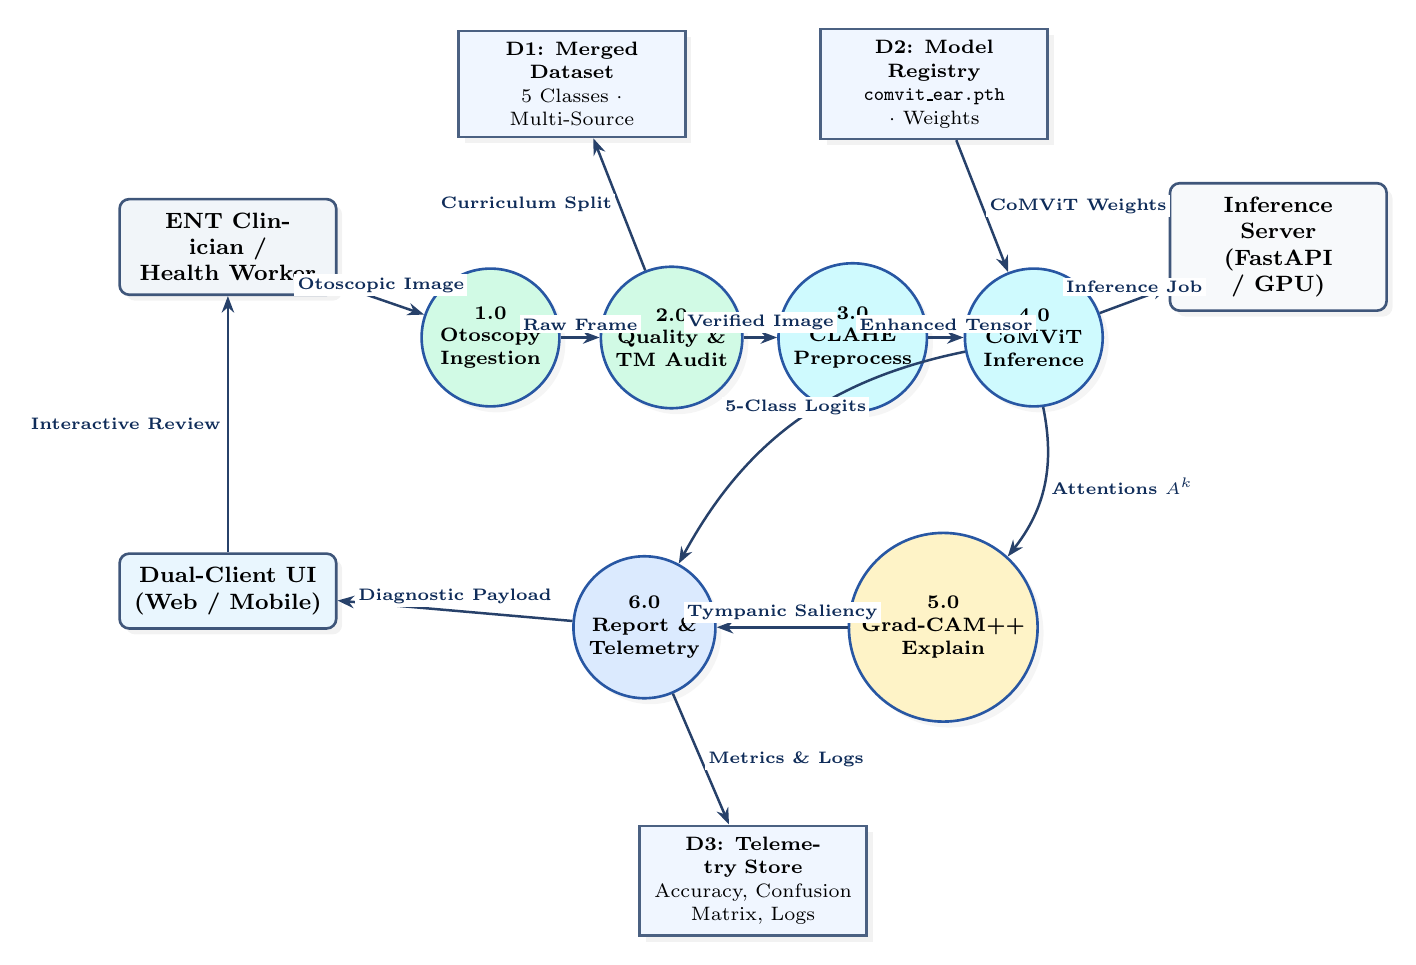
\begin{tikzpicture}[
  x=1.15cm, y=1.15cm,
  font=\sffamily,
  entity/.style={
    rectangle, draw=lavenderDark!80, line width=0.95pt, rounded corners=3.5pt,
    align=center, inner sep=5pt, font=\fontsize{8.0}{9.5}\selectfont\bfseries,
    text width=2.40cm, fill=cInput, drop shadow={opacity=0.10}
  },
  store/.style={
    rectangle, draw=lavenderDark!75, line width=0.95pt,
    align=center, inner sep=4.0pt, font=\fontsize{7.2}{8.5}\selectfont,
    text width=2.60cm, fill=lavenderLight, drop shadow={opacity=0.10}
  },
  proc/.style={
    circle, draw=lavenderMedium!95, line width=0.95pt,
    align=center, inner sep=2pt, minimum size=1.75cm,
    font=\fontsize{7.0}{8.2}\selectfont\bfseries, fill=cStage1, drop shadow={opacity=0.08}
  },
  procblue/.style={proc, fill=cStage4},
  procgold/.style={proc, fill=cStage2},
  prochead/.style={proc, fill=cHead},
  dfdarr/.style={
    -{Stealth[scale=0.85]}, line width=0.90pt, draw=lavenderDark!90
  },
  flowlbl/.style={
    font=\fontsize{6.2}{7.2}\selectfont\bfseries, fill=white, inner sep=1.2pt, text=lavenderDark
  }
]

  % External Entities
  \node[entity] (user) at (-5.8, 3.2) {ENT Clinician /\\Health Worker};
  \node[entity, fill=cStem!70] (client_ui) at (-5.8, -0.6) {Dual-Client UI\\(Web / Mobile)};
  \node[entity, fill=cInput!60] (host_server) at (5.8, 3.2) {Inference Server\\(FastAPI / GPU)};

  % Data Stores
  \node[store] (d1) at (-2.0, 5.0) {\textbf{D1: Merged Dataset}\\ 5 Classes $\cdot$ Multi-Source};
  \node[store] (d2) at (2.0, 5.0) {\textbf{D2: Model Registry}\\ \texttt{comvit\_ear.pth} $\cdot$ Weights};
  \node[store] (d3) at (0.0, -3.8) {\textbf{D3: Telemetry Store}\\ Accuracy, Confusion Matrix, Logs};

  % Core DFD Processes
  \node[proc] (p1) at (-2.9, 2.2) {1.0\\Otoscopy\\Ingestion};
  \node[proc] (p2) at (-0.9, 2.2) {2.0\\Quality \&\\TM Audit};
  \node[procblue] (p3) at (1.1, 2.2) {3.0\\CLAHE\\Preprocess};
  \node[procblue] (p4) at (3.1, 2.2) {4.0\\CoMViT\\Inference};

  \node[procgold] (p5) at (2.1, -1.0) {5.0\\Grad-CAM++\\Explain};
  \node[prochead] (p6) at (-1.2, -1.0) {6.0\\Report \&\\Telemetry};

  % Flow Connections: Ingestion Pipeline
  \draw[dfdarr] (user) -- node[above=1pt, flowlbl]{Otoscopic Image} (p1);
  \draw[dfdarr] (p1) -- node[above=1pt, flowlbl]{Raw Frame} (p2);
  \draw[dfdarr] (p2) -- node[left=1pt, flowlbl]{Curriculum Split} (d1);
  \draw[dfdarr] (p2) -- node[above=1pt, flowlbl]{Verified Image} (p3);
  \draw[dfdarr] (p3) -- node[above=1pt, flowlbl]{Enhanced Tensor} (p4);

  % Model Weights Fetch
  \draw[dfdarr] (d2) -- node[right=1pt, flowlbl]{CoMViT Weights} (p4);
  \draw[dfdarr] (p4) -- node[above=1pt, flowlbl]{Inference Job} (host_server);

  % Inference to Grad-CAM++ and Report
  \draw[dfdarr] (p4) to[bend left=25] node[right=1pt, flowlbl]{Attentions $A^k$} (p5);
  \draw[dfdarr] (p4) to[bend right=25] node[above=1pt, flowlbl]{5-Class Logits} (p6);
  \draw[dfdarr] (p5) -- node[above=1pt, flowlbl]{Tympanic Saliency} (p6);

  % Report to Client UI and Telemetry
  \draw[dfdarr] (p6) -- node[above=1pt, flowlbl]{Diagnostic Payload} (client_ui);
  \draw[dfdarr] (p6) -- node[right=1pt, flowlbl]{Metrics \& Logs} (d3);
  \draw[dfdarr] (client_ui) -- node[left=1pt, flowlbl]{Interactive Review} (user);

\end{tikzpicture}
\end{document}
